% Beamer template
% Author: Ozgur Taylan TURAN
% Delft University of Technology

\documentclass[aspectratio=169]{beamer}
% PACKAGES
\usepackage[english]{babel}
\usepackage{graphicx}
\usepackage{animate}
%\usepackage{calc}
\usepackage{calligra}
\usepackage[absolute,overlay]{textpos}
\usepackage[T1]{fontenc}
%\usefonttheme{serif}
\usefonttheme{professionalfonts}
\usepackage{amsmath}
\usepackage{palatino}
\usepackage{mathpazo}
\usepackage{graphicx}
%\usepackage{subfig}
\usepackage{tikz}
\usetikzlibrary{shapes,arrows}
\usepackage{xcolor}
\usepackage[T1]{fontenc}
%\usefonttheme{serif}
%\usepackage{titling}
\usepackage{graphicx}
\graphicspath{{Figures/}} %Setting the graphicspath
%\usepackage{subfig}
%\usepackage{tikz}
%\usetikzlibrary{shapes,arrows}
\usepackage{mathtools}
\usepackage{cancel}
% CUSTOM PACKAGES
\usepackage{/home/taylanot/texmf/tex/beamerthemetot}
\input{/home/taylanot/texmf/presentation/tune.tex}

 % COVER PAGE INFO   
\newcommand{\mytitle}{\color{White}\huge{\textbf{Meta-Learning Constitutive Laws-Method Development \#1}}}
\newcommand{\mysubtitle}{\color{Pink}\Large{\textbf{Meta-Learning with Kernel Models}}}
\newcommand{\myauthor}{\color{White}\textcalligra{\LARGE Ozgur Taylan Turan}}
\newcommand{\authorlabel}{\small O.T. Turan}
\author{\authorlabel}


\begin{document}
% COVER PAGE

{
\def\beamer@entrycode{\vspace*{-\headheight}}
\setbeamertemplate{frametitle}[default][center]
\setbeamertemplate{navigation symbols}{}
\usebackgroundtemplate{
\includegraphics[width=\paperwidth,height=\paperheight]{cover/coverart.pdf}}

\begin{frame}[plain] 

\begin{minipage}{\textwidth}
	\centering{\mytitle} \\
	%\vspace{1cm}
	%\centering{\mysubtitle} \\
	\vspace{1cm}
	\centering{\color{White}November 15, 2021} \\
	\vspace{1cm}
	\centering{\myauthor}\\
\end{minipage}
\end{frame}
}


\begin{frame}
	\centering
	\mysubtitle
\end{frame}

\section{Recap}
\begin{frame}
  \begin{itemize}
    \item Comments on the writing!
    \item My ideas going forward!
  \end{itemize}
\end{frame}

\begin{frame}{}
  \centering
  \color{Pink}
  Comments on writing?
\end{frame}

\begin{frame}{Going Froward}
  \begin{itemize}
    \item Latent Variable Models (Maybe a bit later?)
    \item Meta-learning with KernelRidge?
  \end{itemize}
\end{frame}

\begin{frame}{Meta-learning with Kernel Ridge}
  \begin{itemize}
    \centering
  \item We are after $f\in \mathcal{F}$, where $\mathcal{F}$ is a class of functions 
  \item Non-parametric Representer Theorem states that $f$ that minimizes regularized risk functional $\mathcal{L}+g(||f||)$ (note, $||\cdot||$ is in RKHS) is given by $f(\cdot)=\sum_{i=1}^{N}\alpha_i k(\cdot,\mathbf{x}_i)$, where $N$ is the number of training samples $\{\mathbf{x}_i, y_i\}_{i=1}^{N}$
  \end{itemize}
\end{frame}

\begin{frame}{Meta-learning with Kernel Ridge}
  \begin{itemize}
    \centering
  \item We are after $f\in \mathcal{F}$, where $\mathcal{F}$ is a class of functions 
  \item Non-parametric Representer Theorem states that $f$ that minimizes regularized risk functional $\mathcal{L}+\Omega(||f||)$ (note, $||\cdot||$ is in RKHS) is given by $f(\cdot)=\sum_{i=1}^{N}\alpha_i k(\cdot,\mathbf{x}_i)$, where $N$ is the number of training samples $\{\mathbf{x}_i, y_i\}_{i=1}^{N}$
  \end{itemize}
\end{frame}

\begin{frame}{What I was trying to do?}
  \centering
    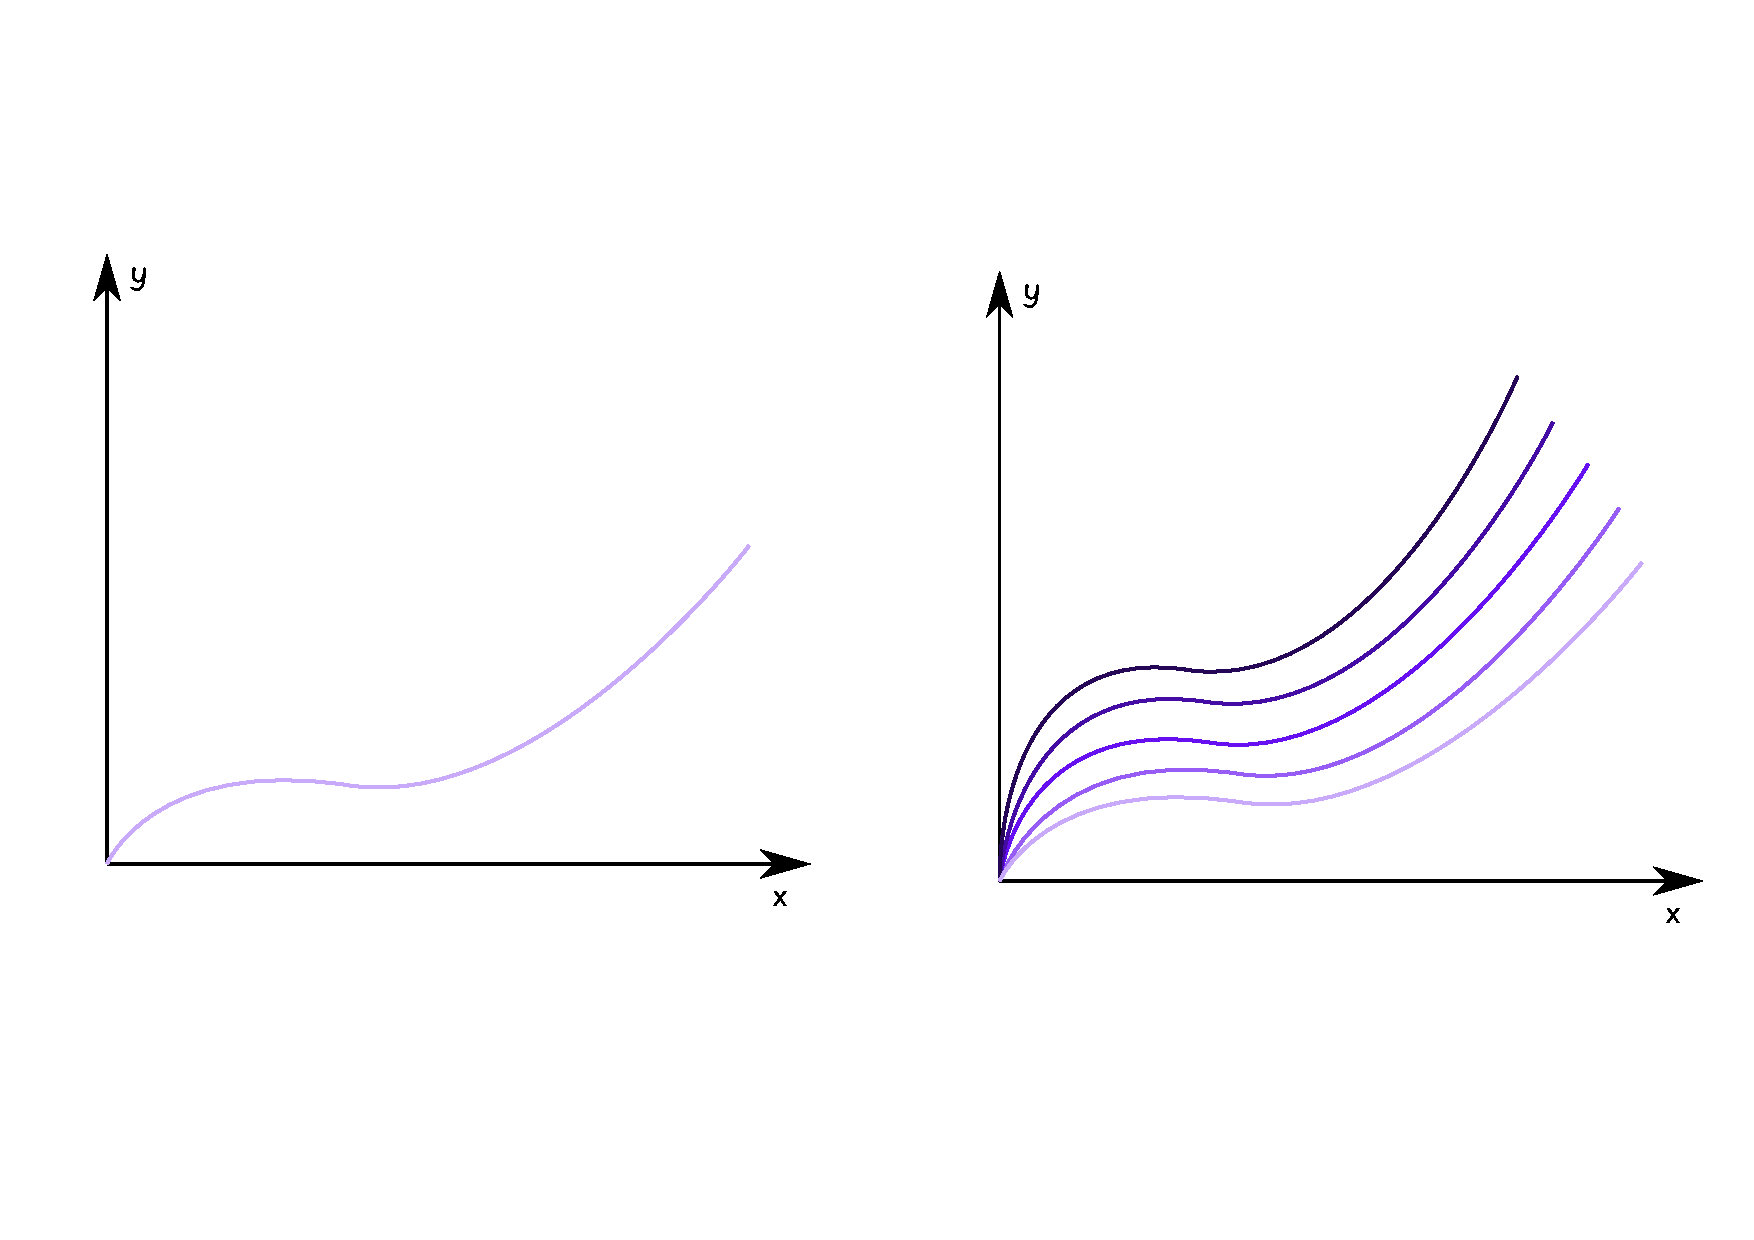
\includegraphics[width=0.8\textwidth]{singlevsmeta}
\end{frame}

\begin{frame}{2-Options\cite{Scholkopf2002}}
  \centering
    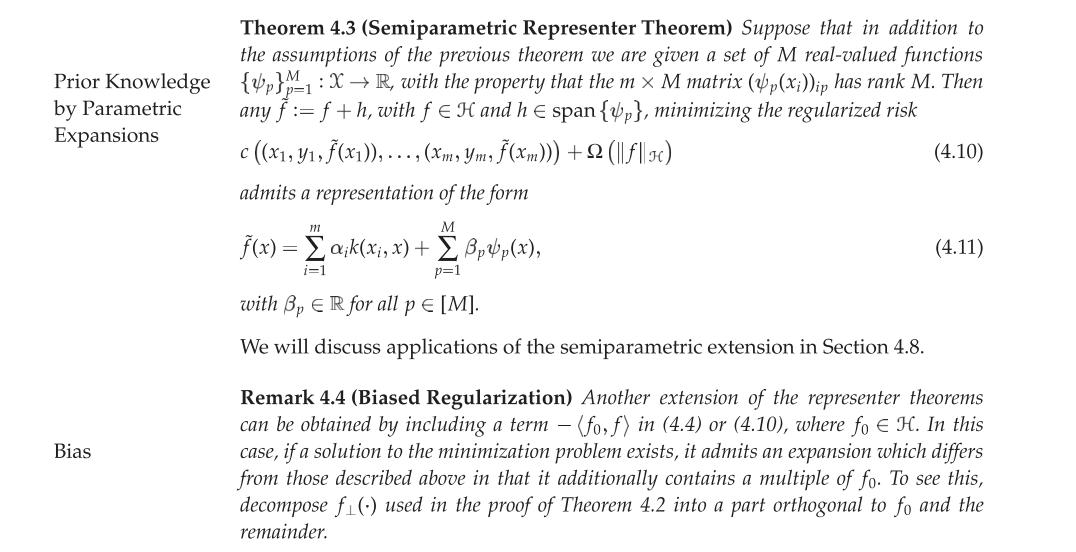
\includegraphics[width=0.8\textwidth]{options}
\end{frame}

\begin{frame}{2-Options\cite{Scholkopf2002}}
  \begin{itemize}
    \item Biased regularization framework similar to $\cite{Denevi2018}$ in a nonlinear setting. (They just mention that it is doable and do not show explicitely.)
    \item Semi-parametric definition is also interesting. 
  \end{itemize}
\end{frame}

\begin{frame}{Literature}
  \begin{itemize}
    \item Could not find anything similar in these ranges.
  \end{itemize}
\end{frame}

\begin{frame}{What shall we do?}
  \begin{itemize}
    \item Could not find anything similar in these ranges.
  \end{itemize}
\end{frame}

\end{document}
